% Analysis section
In this section we will outline the process used for each of the clustering methods.
An aim of this work was to help astronomers determine which filters were best at identifying different types of objects in a survey. 
Since the average survey is limited to four filters, different combinations of four filters were used to construct colours for clustering. 
Colours were constructed using the difference between two wavelengths. For a given combination of four filters, all possible colour combinations were used. % Change as needed
The feature space was constructed in two and three dimensions, to add a layer of analysis that isn't typically found in colour-colour space.

\subsection{Clustering Process}
Clustering was performed using all three methods for each colour combination. 
The methods were used independantly and in unison in order to determine the optimal clustering.
The following process allowed the investigation of the effect of all paramters on each clustering technique, leading to an optimal clustering. 
\begin{enumerate}
\item \textbf{Mean-Shift:} Mean-Shift clustering was performed first by estimating the bandwidth paramter with the $estimate_bandwidth$ function in $scikit_learn$.
Following the initial clustering, a "bandwidth hierarchy" was created by performing the clustering again with bandwidth values between $\pm$ intervals of $0.1$ from the estimated bandwidth.

\item \textbf{AP:} Affinity Propagation clustering was then performed by setting the preferences to 10\% of the number of objects in the data set, and setting the damping factor to $0.95$.
Following that clustering, an "Affinity hierarchy" was created by varrying the damping factor, and preference value to determine the effect of each parameter. 

\item \textbf{K-Means:} K-Means clustering was performed last.
The first two clusterings were performed using the number of clusters determined from the initial clusterings by Mean-Shift and AP.
Next, K-Means was performed with $K = \pm 4$ from the original clustering.
\end{enumerate}
\subsection{Selecting the Clustering}
In order to determine the optimal clustering, a series of metrics were used.
For each clustering, the silhouette score, cluster centers, root mean square, average and standard devation of each colour, and the distances between points in each cluster were calculated. 
\subsubsection{Silhouette Score}
The silhouette score is a metric used to describe the compactness of a cluster in a given clustering and is calculated as an average of all samples in a clustering.  
The silhouette score is given by:
\begin{equation}
\label{eq:ss}
Silhouette Score = \frac{b - a}{\textit{max}\big(a, b\big)}
\end{equation}
where $a$ is the mean intra-cluster distance, and $b$ is the distance between a point and the nearest cluster that point is not a member of.
In addition to the average score of the clustering, the average score for each cluster within the clustering was computed.
The cluster score determines what is driving the average score, and uncovers which clusters are most compact.

\subsubsection{Cluster Statistics}
Various statistics were calculated for each cluster within a clustering to help describe the similarity between the objects in a given cluster.
The standard deviation and average colour was calculated for each colour and each cluster within a clustering. 
These metrics describe the distribution of the objects in the colour-colour space within a cluster. 
Clusters that had large standard deviations were viewed as too dissimilar to be a meaningful cluster, and the clustering parameters were changed or the clustering was removed. 
Clusters whose averages and medians were not close were also discredited. 

The fractional sizes of each cluster were also calculated.
This metric describes the distribution of objects between clusters, and provided a complete way to evaluate a given clustering. 
If a clustering segmented the objects into a large cluster followed by several smaller ones, the clustering was investigated further, as this segmentation could mean one of two things. 
This type of clustering could be a result of the identification of interesting objects, in which case the clustering algorithm was able to identify the objects and place them in the same cluster.
However, this type of clustering could also be a result of the underlying distribution of the data, as the clustering techniques are largely drawn to areas of high density.
If this is the case, the clustering only created the smaller clusters as a result of the parameters imposed on the clustering.

\subsubsection{Parameter Relationships}
In addition to metrics, the relationships between various metrics were investigated to determine the optimal clustering.
Figure~\ref{fig:sscore} shows the relationship between the silhouette score and the number of clusters imposed on the data for each type of clustering. 
The optimal number of clusters is found where the relation flattens.
For K-Means, this point is between 5-10 clusters.

\begin{figure}[H]
\centering
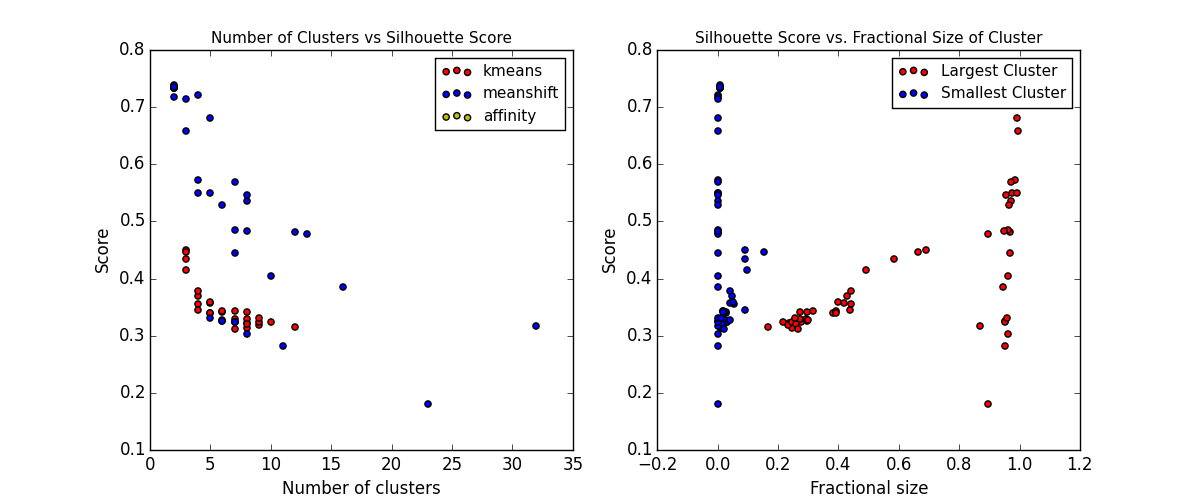
\includegraphics[width=\linewidth]{figs/silhouette_score_relation}
\caption{Distribution of the silhouette score as a result of the number of clusters imposed. The \textit{blue} points are the scores of Mean-Shift clustering, \textit{red} points are scores of K-Means, and \textit{yellow} points are scores of AP.}
\label{fig:sscore}
\end{figure}

The Mean-Shift scores do not follow a similar distribution as K-Means, as the accuracy of Mean-Shift is more directly related to the bandwidth parameter, seen in Figure~\ref{fig:bwscore}.
The optimal Mean-Shift clustering was chosen by finding the bandwidth where the relation between the bandwidth and number of clusters reached an elbow, which was usually between 3 - 5 clusters.

\begin{figure}[H]
\centering
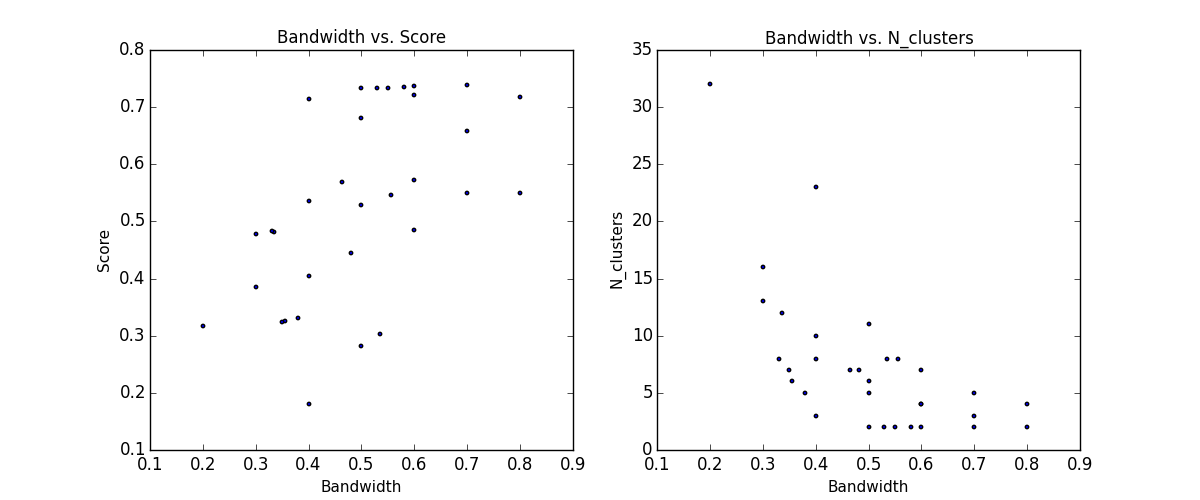
\includegraphics[width=\linewidth]{figs/meanshift_parameters}
\caption{Distribution of the silhouette score as a function of bandwidth, and the distribution of the number of clusters as a function of bandwidth.}
\label{fig:bwscore}
\end{figure}
